\documentclass[12pt]{article}
\usepackage{arydshln}
\usepackage{multirow}
\usepackage{graphicx}
\usepackage{bm}
\usepackage{float}
\usepackage{amsmath}
\usepackage{amssymb}
\usepackage{color}
\usepackage{caption}
\usepackage{subcaption}
\usepackage{mathrsfs}
\usepackage{mdframed}
\usepackage[margin=2cm]{geometry}
\usepackage[superscript,nomove]{cite}
\numberwithin{equation}{section}
\numberwithin{figure}{section}
\usepackage[makeroom]{cancel}
\usepackage{textcomp}
\usepackage{gensymb}
\DeclareMathOperator\arctanh{arctanh}
\usepackage[colorlinks=true]{hyperref}
\usepackage{cleveref}
\crefdefaultlabelformat{[#2#1#3]}
\begin{document}
\renewcommand\citeform[1]{[#1]}
%
\title{MSc Data Science Project: Can a Convolutional Neural Network judge a book by its cover?}
\author{\\Ryan Hill MSci\\\\
Supervisor: Dr Hubie Chen\\\\
Birkbeck, University Of London\\\\
\texttt{rhill06@mail.bbk.ac.uk}}
\date{\today}
\maketitle
\thispagestyle{empty}
\graphicspath{{images/}}
\begin{abstract}
	In this work we revisit and build upon the work of Iwana et al.\cite{KenjiIwana} in an attempt to use convolutional neural networks (CNNs) to predict the genre of a book based entirely on its cover image. We test various pre-processing methods for the images and use a selection of newer, more complex, CNNs to attempt to improve on the results of the previous work. Using an Inception-ResNet-v2 we achieve Top-1 accuracy of 24.7\% and a Top-3 accuracy of 45.4\% which is an improvement over previous results.
\end{abstract}
\renewcommand{\abstractname}{Acknowledgements}
\begin{abstract}
Thank you to Pete Stewart and Openreach Ltd for sponsoring this degree, and thank you David, Scott, and Craig who made working while studying a little easier and less stressful than it would have been otherwise. Thank you to my friends who have put up with me over the last 2 years. Finally most of all I want to thank my parents, who have always supported me and my learning, even though it has been a long time since they understood any of it. 
\end{abstract}

\begin{figure}[!b]
	\centering
	
\includegraphics[scale=0.4]{bbk_logo.jpg}
\end{figure}

\clearpage
%
{\hypersetup{linkcolor=black}
\tableofcontents}
\thispagestyle{empty}
\clearpage
%
\setcounter{page}{1}
\section{Introduction} 
\label{sec:intro}
Convolutional neural networks (CNNs) have been used for image classification for the last 30 years\cite{Cun1989}, with ever more accurate, and more complex, model architectures being produced and tuned on benchmark datasets. CNNs have been used to identify clothing types, objects, music, and even identify artists of paintings; but as far as we are aware only once has someone tested asked the question of the ability of a CNN to judge a book by its cover i.e. predict the genre of the book based on the cover image. We will discuss the work of this person in \cref{sub:Related Works}. 

The question of predicting a genre based only on a cover image is more difficult than it may first appear; many books at least slightly span genres, and designs are at their heart art which means some personal interpretation will always play a part. Being able to successfully build a model to solve this problem would allow designers to use such a tool to ensure that a design is clear to their target audience, it could allow some data-validation of book related data, and could help uncover some underlying design principles in genre classification that is not evident to us currently. 

In this work we attempt to train a selection of modern CNN architectures that have been pretrained on the ImageNet dataset to correctly predict the genre of a book from its cover image. The remainder of this work is structured as follows; in the rest of this section we discuss related works, then in \cref{sec:Theory} we discuss some theoretical concepts that we use within the work for those familiar with Machine Learning but not in CNNs. In \cref{sec:Data_collection_and_pre-processing} we present our methods of the adjustment of the existing datasets and the testing of different methods of pre-processing the images. \Cref{sec:Model_Training} contains the information about how we configured and trained the models, followed by the evaluation of our results and discussion of next steps in \cref{sec:Evaluation_and_Further_Exploration} before summarising our work in \cref{sec:Conclusion}. Please note in this work we will use the terms \emph{class, genre, classification,} and \emph{category} interchangeably to describe the genre that a particular book cover belongs to.

\subsection{Related Works} 
\label{sub:Related Works} 
So far as we can tell at the time of writing there is only one piece of prior work that has been completed in the area of predicting book genres based on their cover images; the work published by Iwana et al.\cite{KenjiIwana}. In their work they produced 2 datasets, the \emph{Book32} dataset and the smaller, balanced, dataset known as \emph{BookCover30}. These datasets are the best collection of cleaned data that are readily available and we use these within our work, with some small adjustments as discussed in \cref{sub:Image Download and Manual Review}. In their work they trained 2 CNNs, LeNet and AlexNet on the BookCover30 dataset, achieving 13.5\% and 24.7\% Top-1 accuracy respectively; more detailed information of their results is available in \cref{tab:results_acc}.

They go on in their work to discuss the results of their models with analysis and call out few cover design principles including the use of colour, objects, and text. We further investigate the colour angle in \cref{sub:Further_Analysis}.

Our work builds atop theirs by using more modern and complex CNNs to attempt to identify if the more powerful architectures are more capable of producing equivalent or improved results whilst training for significantly fewer epochs than the original paper.
% subsection Related Works end 
% section CNN Theory and Architectures
\section{Theory} 
\label{sec:Theory} 
Whilst in this work we do not detail the full design (beyond that provided in \cref{sec:CNN_Architectures}) and reasons for those designs of the models we will use, it may be beneficial for the reader to understand some concepts of neural networks in particular the components that make up convolutional neural networks. In this section we briefly describe some of these components as well as some of the other methods used within this work in \cref{sub:Transfer_Learning,sub:Activation_Maximisation}. We assume the reader already has familiarity with introductory machine learning concepts such as backpropagation and fully connected neural networks.
\subsection{Components of Convolutional Neural Networks} 
\label{sub:Components_of_Convolutional_Neural_Networks} 
\subsubsection{Activation functions}
Most layers of a neural network have some kind of activation function (a function that transforms the output of the neuron before passing it to the next layer); these are used to ensure both that there is at least some level of activity, and also to place the values within a specific range (usually networks only take in values between 0 and 1 so they need to be in this range). Some normalisation is also usually applied which is discussed later. For our purposes there are only 3 activation functions that are relevant for this work.

Linear activation is exactly what it sounds like, there is no transformation to the output. Rectified Linear Unit (ReLU) is a function that returns the input when the value is greater than or equal to zero, and zero otherwise. Finally, softmax is used almost exclusively in the final layer of a network to transform the outputs into values that sum to 1 (to be interpreted as the probability of that record belonging to the class that neuron represents). These are defined mathematically in \cref{eq:act_linear,eq:act_relu,eq:act_softmax}.

\begin{align}
	f_{linear}(x) &= x \label{eq:act_linear}\\
	f_{ReLU}(x)   &= \max(0, x) \label{eq:act_relu}\\
	f_{softmax}(\bm{x})_i &= \frac{e^{x_i}}{\sum_{\alpha=1}^{K}{e^{x_\alpha}}}\label{eq:act_softmax}
\end{align}
Where the non-bold $x$s are just individual outputs, but the softmax function requires all K outputs of the layer for calculation. Technically, most pre-built models in Tensorflow use ReLU6 as opposed to pure ReLU, this version is shown in \cref{eq:act_relu6}.
\begin{equation}
	f_{ReLU6}(x) = \min(\max(0, x), 6) \label{eq:act_relu6}
\end{equation}

\subsubsection{Convolutional layers}
A convolutional layer  is different to the traditional fully connected layers and is used predominantly in image classification, forming the fundamental building block of a CNN. A convolutional layer is defined by 3 key parameters, and the additional choice of padding. The 3 parameters that define a basic convolutional layer are the number of filters (analogous to the number of neurons in a dense layer) which is also the number of channels the output of that convolution will have, the size of the filters, and the stride (or step size) of the filter. 

A filter (also called a kernel) is applied atop of the input, starting at the top left of the input, and pointwise multiplication is applied to each set of elements, then their sum is computed. In the case of multiple input channels the same filter is applied over all channel and their outputs are summed. This value is the the output value of the top left cell of the output tensor. The filter is then moved left by the number of elements defined by the stride; when the end of the row has been reached the filter is moved down by the same stride. This process is repeated until the filter has been applied to the entire input. Once all filters have been applied this set of outputs is referred to as the feature map. This process is demonstrated in \cref{fig:conv_process} and quantified mathematically as

\begin{equation}
	m_{i,j,k} = \sum_{\chi = 1}^{C}\sum_{\alpha = 1}^{l}\sum_{\beta = 1}^{l} f_{\alpha,\beta, k} \times x_{(\alpha +(i-1)*s), (\beta + (j-1)*s),\chi}
\end{equation}
where $m_{i,j,k}$ is the component of the feature map $\bm{m}_k$ for output channel $k$ at position $(i, j)$, C is the number of channels in the input, $x$ is the 3 dimensional input tensor (height, width, and channels) input, $f$ is the $k^{th}$ filter of size $l\times l$, and $s$ is the stride. The complexity of the subscripts on $x$ arises from the need to describe the offset provided by the size and stride of the kernel. We apply this equation for the examples given in \cref{fig:conv_process} in the following, noticing the simplifications that $C = s = 1$ so that $k \subseteq \{1\}$, and in this case $l = 3$. Then for the examples given in the image we have
\begin{align}
	m_{1, 1, 1} &= \sum_{\alpha = 1}^{l}\sum_{\beta = 1}^{l} f_{\alpha,\beta, 1} \times x_{(\alpha +(1-1)), (\beta + (1-1)),1}	\\
	m_{1, 1, 1} &= (1\times1 )+ (0 \times 2) + (1 \times 1) + (0 \times 2) + (1 \times 0) + (0 \times 0) + (1 \times 1) + (0 \times 0) + (1 \times 2) = 5 \\
	m_{1, 2, 1} &= \sum_{\alpha = 1}^{l}\sum_{\beta = 1}^{l} f_{\alpha,\beta, 1} \times x_{(\alpha +(1-1)), (\beta + (2-1)),1}	\\
	m_{1, 2, 1} &= (1\times 2)+ (0 \times 1) + (1 \times 1) + (0 \times 1) + (1 \times 0) + (0 \times 1) + (1 \times 0) + (0 \times 2) + (1 \times 1) = 3 \\
	\vdots \nonumber	\\
	m_{3, 3, 1} &= \sum_{\alpha = 1}^{l}\sum_{\beta = 1}^{l} f_{\alpha,\beta, 1} \times x_{(\alpha +(3-1)), (\beta + (3-1)),1}	\\
	m_{3, 3, 1} &= (1\times 2)+ (0 \times 1) + (1 \times 0) + (0 \times 0) + (1 \times 2) + (0 \times 1) + (1 \times 1) + (0 \times 0) + (1 \times 2) = 7
\end{align}
Note that in the image the kernel is displayed second visually but due to the order we wrote the equation is in the kernel elements are on the left of the multiplication.



In total for a square input and kernel this leads to an output of the dimensions described by

\begin{equation}
	\label{eq:feat_map1}
	\dim(\mathscr{M}) = \left[\frac{m-f}{s} +1 \right] \times \left[\frac{m-f}{s} +1 \right] \times n_{f}
\end{equation}
where $\mathscr{M}$ is the full feature map, $m$ is the width and height of the input, $f$ is the width and height of the filter, $s$ is the stride, and $n_f$ is the number of filters.

Using this method it means that, unless the filter size and stride are both equal to 1, certain parts of the input will never be exposed to the centre of the filter, and the output of the process will always lead to a smaller size. This can be an issue when multiple convolutional layers are applied in sequence as whilst the number of channels may increase the size of each channel will decrease. An approach that removes this problem is to first pad the input with 0s on all sides, the size of the padding being determined by the goal output size as well as the filter size and stride. By applying padding the output size of the image changes from that described in \cref{eq:feat_map1} to instead be
\begin{equation}
	\label{eq:feat_map2}
	\dim(\mathscr{M}) = \left[\frac{m+2p-f}{s} +1 \right] \times \left[\frac{m+2p-f}{s} +1 \right] \times n_{f}
\end{equation}
where $p$ is the padding size on one side.


\begin{figure}
	\centering
	\captionsetup{justification=centering}
	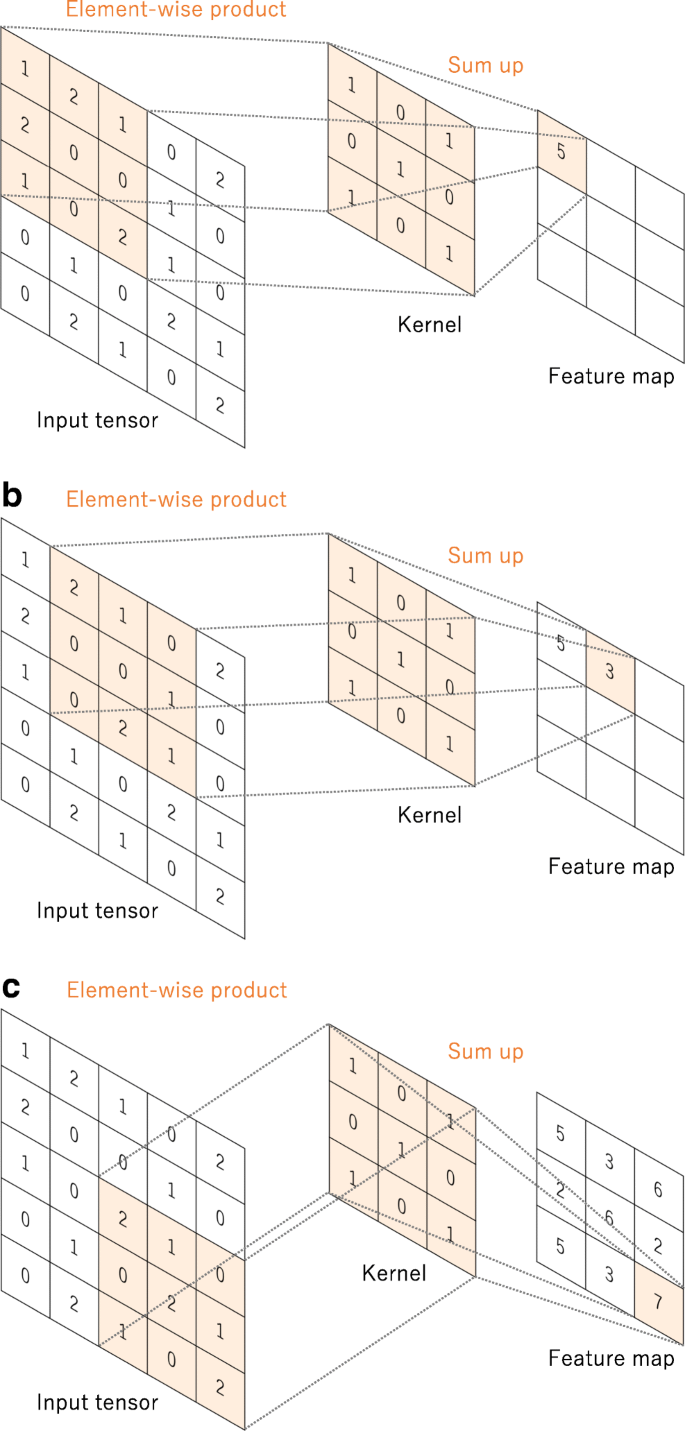
\includegraphics[scale=0.25]{cnn_application.png}
	\caption{An example of a 3x3 filter being applied to a single channel input, with stride of 1 and 0 padding. \cite{Yamashita2018}}
	\label{fig:conv_process}
\end{figure}

Whilst the number of filters, filter size, and stride are hyperparameters that must be set by the user, the actual values of each filter in the layers are learned as part of the backpropagation training of the network.


\subsubsection{Depth-Wise Convolutions}
Depth wise convolutions are similar to normal convolutional layers in all ways except one; instead of applying the filter to each channel of the input and summing the outputs to produce a single output channel we instead keep these outputs separate and produce an output with as many channels as the input per filter.  When followed by a 1x1 convolution (also known as a pointwise convolution) this has the effect of merging the layers via addition and combined these two processes actually have a reduced computational cost when compared to a traditional convolution \cite{Sandler2018}. The results from depth-wise convolutions are identical to traditional convolutions but due to this improvement in computational cost they are used within many complex models to improve performance. 

\subsubsection{Pooling}
Pooling is an operation used within convolutional neural networks to reduce the size of channels/feature maps within the network. Pooling is applied using the same size and stride arguments as convolutions however instead of pointwise multiplication they aggregate across their area. These operations tend to either be maximum or average and are determined either by the user or the CNN architecture. These are applied per-channel and no aggregation across channels is completed afterwards. The dimensions of the output after pooling can be calculated using the same method as before displayed in \cref{eq:feat_map2}. Traditionally (and in our work) pooling is completed with no padding. Global pooling refers to when the size of the filter matches the size of the input and a 1x1xdepth output is returned. For example global average pooling on the output feature map of \cref{fig:conv_process} would be a 1x1 result of 7, global average pooling would give 4.333\dots and max pooling of size 2x2 with a stride of 1 would lead to
$$
\begin{bmatrix}
	6 & 6 \\
	6 & 7 \\
\end{bmatrix}
$$
as where average pooling of the same size and stride would result in
$$
\begin{bmatrix}
	5.25 & 4.25 \\
	5.25 & 4.5 \\
\end{bmatrix}
$$

\subsubsection{Batch Normalisation}
Batch normalisation was introduced in a 2015 paper by Sergey Ioffee and Christain Szegedy\cite{Ioffe2015} and is a step introduced into neural networks, including CNNs, between the layers and the activation functions. Batch normalisation works by applying re-scaling and re-centering transformations to the output of a layer i.e. transforming the output of that layer for that batch to have a mean of 0 and a standard deviation of 1. This has the effect of greatly reducing training time and increases accuracy by way of reducing the change in the data distribution between different layers and more importantly reducing the change of this over time via backpropagation. 

\subsubsection{Residual Networks}
Residual networks (ResNets) were introduced by He et al. in 2015\cite{He2015a} to allow for far deeper networks than previously used. The basic premise is that the layer input forms part of the output directly via a scaled addition to the convolved, normalised, and activated output. This allows for information to be carried further through the network and was shown to achieve better results against benchmark image classification datasets. Further detail and formulation is available in the original paper so we do not reproduce that here as a grasp of the main concept is all that is required.

% subsection Components_of_Convolutional_Neural_Networks end 
\subsection{Transfer Learning} 
\label{sub:Transfer_Learning} 
Transfer learning is a concept in machine learning that \emph{knowledge} gained by a network in one domain could be used within another domain, either out of the box or as a starting point for training. In our case, the models we use have already been trained on the more complex ImageNet dataset so would be suitable to use in transfer learning to save a lot of time training the model from scratch.


In transfer learning it is possible to take one of two approaches; the first is to use the existing model weights and biases as a starting point for training and to train the entire model using your training data, the second is to freeze the weights and biases for the feature engineering part of the model i.e. all but the fully connected layers at the end, and just train the classification top of the model. In our work we took the second approach as, given the size of the models we are using, training the full model would have been computationally expensive, and given the relatively small amount of training data would also have, when compared to the number of parameters in the model, been unlikely to have improved accuracy.
% subsection Transfer_Learning end 

\subsection{Activation Maximisation} 
\label{sub:Activation_Maximisation} 
Activation maximisation is a technique that can be applied to neural networks, in particular CNNs, to help understand what an idealised input for a given output the network would expect. Is is often combined with saliency or attention maps to identify the area(s) of a specific image that the CNN is drawing on for the classification. Activation maximisation is used instead to produce an input for the network that maximises the activation of the target class. 

Given the potentially complex networks that can be reviewed using this technique the theory itself remains quite simple in nature. Given a trained model, as defined by the architecture and parameters, that ends with a fully connected dense layer the first step is to freeze all the parameters for the model i.e. the weights and biases. Next, the activation function in the final layer (most likely a softmax function) should be replaced with a linear function instead. The reason for this replacement is subtle but important; due to the softmax function taking as an input the entire vector of values it is possible to maximise a single value by minimising the other values. If we were to continue to use the softmax it could be the case that in trying to generate an image that most represents class A, we instead generate an image the least represents all other classes; by using a linear activation instead we avoid this issue entirely.

Finally, a random input, $\bm{x}$ is chosen at the start and is evolved using backpropagation using the learning rule defined as

\begin{equation}
	\label{eq:act_max}
	\Delta x_i = -\eta\frac{\partial \hat{y}_t}{\partial x_i} + \mathcal{R}
\end{equation}
where $\eta$ is the learning rate which in this work was set at 1, $\mathcal{R}$ is any regularisation terms, and $\hat{y}_t$ is the activation value of the target class. Simply put, change the values for the input in a way that increases the activation for that class within some constraints. One regularisation term used in this work is L2norm. It is defined as the root mean squared value of the vector and in this case helps ensure to generate a smooth image, penalising edges.
% subsection Activation_Maximisation end 
% section Theory end 
\section{Data collection and pre-processing} 
\label{sec:Data_collection_and_pre-processing} 
\subsection{Image Download and Manual Review} 
\label{sub:Image Download and Manual Review} 
The 207,572 images within the complete book32 dataset covering all original 32 classes were downloaded at full resolution using a slightly altered version of the script provided within the Iwana repository \cite{iwanarepo}. The original csv containing all image URLs was split into files of no more than 20,000 records each to allow the downloads to be run over multiple sessions due to the slow data transfer rates. The overhead of reading data between Google Drive and Google Colab meant that even checking before downloading an individual file if it already existed was not much faster than downloading and writing the file anyway. Each sub-file was then iterated over using the remainder of the original script, downloading each image into a sub-folder of the class for that image i.e. the genre classification. Once all images were downloaded a sample few were manually checked to verify as best as possible that the data was still correct and the downloads has worked. 

At this point we attempted to identify if any records used in the bookcover30 train or test datasets were actually boxsets, and as such would likely have an unrepresentative cover image, an example of such an image can be seen in \cref{fig:bad_cover}. The terms used in a regex search of the titles were \emph{``boxed set'', ``boxset'', ``box set'', ``anthology'', ``bundle'', ``\#-book'', and ``\# book''}. 264 records within the bookcover30 dataset matched at least one of these terms and were extracted into a new folder for manual review. The process was somewhat subjective but as a rule of thumb we rejected any image that was not a single front facing cover or that contained pictures of multiple books and was not an arrangement of covers; single covers that seemed to be specifically designed for a boxset were considered acceptable. In total 94 records needed to be removed due to these rules. To preserve the class balance of the train and test datasets, new records were chosen from the book32 dataset by making like-for-like swaps of the same class; any new covers were also reviewed to ensure they were not boxsets. No verification of the class assignment to images was performed so any errors that existed in the original data would have persisted and we continue to use the single class chosen by the original authors in the case of multi-class books.

\begin{figure}
	\centering
	\captionsetup{justification=centering}
	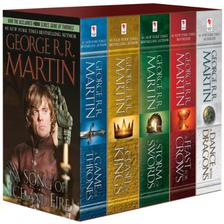
\includegraphics[scale=0.5]{0345535529.jpg}
	\caption{An example of a rejected \emph{``cover''} image as it did not meet our criteria.}
	\label{fig:bad_cover}
\end{figure}

We chose to split the training data out into training and validation data using a 90/10 random split per class to ensure class balance in all of the training, validation, and test sets. In total the training set compromised of 46,170 records, the validation set 5,130 records, and the test set 5,700 records; with 1,539, 171, and 190 records per class respectively. 

% subsection Image Download and Manual Review end 
\subsection{Image Pre-processing Technique} 
\label{sub:Image_Pre-processing_Technique} 

We next used 3 different image preparation methods on the datasets to attempt to identify the method that would lead to the best accuracy within our models. At this stage all methods output an image of 299x299 pixels as this was the largest size we would need for any future models. By reducing the image size twice, first now and then again when using a specific model, we were potentially losing some information that would lead to a less accurate model; however we chose to do this to speed up training and testing by having to load much smaller data in compared to the original full sized images. Before pre-processing was done we collected the initial shape and average RGB values of each image for further analysis later in \cref{sub:Further_Analysis}.

The first pre-processing method (\emph{NoPrep}) was to simply rescale the image directly down to a 299x299 shape using inter-cubic interpolation. This method uses a 4x4 neighbourhood around the new pixel location to smooth the transition between boundaries as smoothly as possible and the implementation in the \emph{opencv} python library was used throughout. This was chosen at the time as a common all-purpose interpolation method, however after later research this method is often chosen to enlarging images, not shrinking them so the potential to use a better interpolation method (e.g. inter-area) could be used in future work.

The second method (\emph{Padded}) was to first pad the images with a symmetric pure white border on either the left/right or top/bottom depending on if the image was portrait or landscape (no padding was done if the image was already a perfect square). These images were then downscaled to 299x299 using the same method as above. The final method (\emph{Cropped}) was to crop the image to a perfect square before the same downscaling method was used. 

Once the images had been processed we used a MobileNetV2 model on each processed training and validation dataset for 30 epochs with an early stopping patience of 15 (i.e. if no improvement was seen in validation accuracy over 15 epochs then we did not continue) and the best model for validation accuracy was kept. The model was trained using the default TensorFlow 2 settings of the adam optimiser with a loss function of sparse categorical cross entropy. More details of the set up are detailed in \cref{sec:Model_Training} as other than the epoch and early stopping the same configuration was used for the main training process. The progress on the training and validation data can be seen in \cref{fig:prep_perf} and the test results of this model trained on each of the 3 datasets is presented in \cref{tab:preprocres}. The second method, padding the image with a white border, achieved the best result on the test data of 15.81\% accuracy. 

\begin{figure}
	\centering
	\captionsetup{justification=centering}
	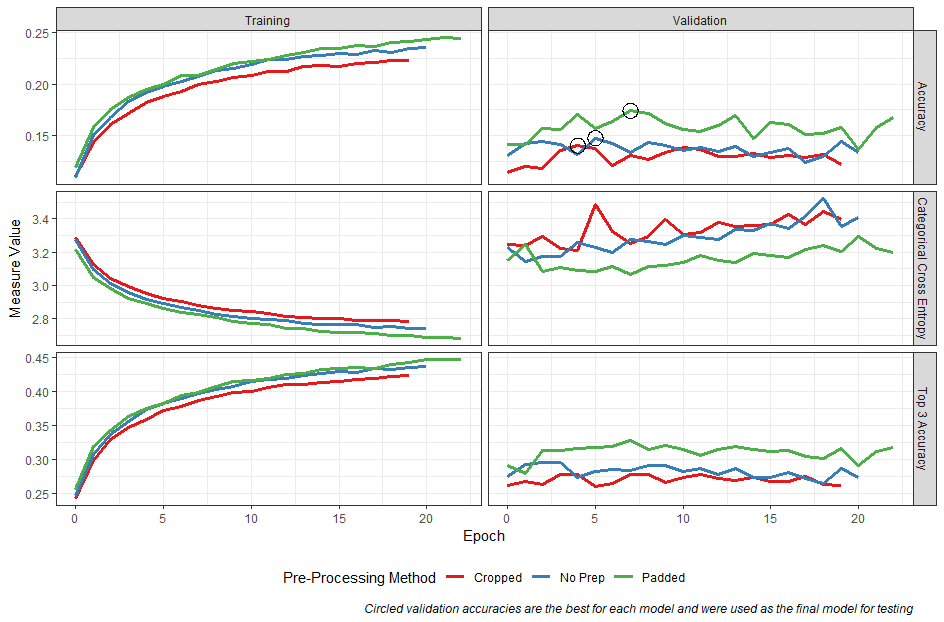
\includegraphics[scale=0.5]{prep_training.png}
	\caption{Performance of different pre-processing methods throughout training of MobileNetV2}
	\label{fig:prep_perf}
\end{figure}


\begin{table}[]
	\centering
	\begin{tabular}{|l|r|r|}
	\hline
	\textbf{Pre-processing Method} & \multicolumn{1}{l|}{\textbf{Best epoch}} & \multicolumn{1}{l|}{\textbf{Test Accuracy}} \\ \hline
	NoPrep                         & 8                                        & 14.39\%                                     \\ \hline
	Padded                         & 6                                        & 15.81\%                                     \\ \hline
	Cropped                        & 5                                        & 12.88\%                                     \\ \hline
	\end{tabular}
	\caption{Results of short training on MobileNetV2 on different image pre-processing methods}
	\label{tab:preprocres}
\end{table}

It is important to note at this point that just because this method achieved the best result for this model in a short number of epochs is no guarantee that this would be the method that achieves the best results in other models or over longer epochs. We use this as a rough benchmark as given the constraints on computing power available to us we were only able to train each model in \cref{sec:Model_Training} once for a reasonable number of epochs, so a decision had to be made. It is also possible that hyperparameter tuning for each of these datasets may have led to different outcomes, but again due to the constraint on resources we decided it best to use domain accepted defaults and as such we progress with the padded dataset.

% section Image_Pre-processing_Technique end 
% section Data_Collection_and_pre-processing end 
\section{Model Training} 
\label{sec:Model_Training} 
\subsection{Configuration} 
\label{sub:Configuration} 
All model architectures consisted of their respective base CNN structure as detailed in \cref{sec:CNN_Architectures} followed by a global average pooling 2D layer to reduce the dimensionality of our tensor and to ensure a flat 1D vector, this is then fully connected to a 30 neuron output layer with a softmax activation. All models were also trained using the same setup in terms of hyperparameters, optimisers and loss functions; the loss function was sparse categorical cross entropy (sparse due to the usage of a non one-hot encoded target vector), the optimiser was the Adam optimiser \cite{Kingma2015}. The optimiser was used with default hyperparameters as defined within the TensorFlow implementation, the most important being the learning rate with was left at the initial value of 0.001. The reason for the usage of the default hyperparameters and not using a more advanced custom optimiser, such as WAME \cite{Mosca2017}, was due to the constraints on access time to computing power. As is the training already had to be completed across multiple sessions and doing any tuning would have resulted in too large a time required to produce meaningful results; Adam produces decent results with the defaults and so they were used in this work.

The models themselves, MobileNetV2 \cite{Sandler2018}, Inception-ResNet-v2 \cite{Szegedy2016}, and ResNeXt50 \cite{Xie2016} were chosen to represent a wide spread of model capabilities and complexities as highlighted in Figure 1 of the Benchmark Analysis of CNNs completed by Bianco et al\cite{Bianco2018}. MobileNetV2 was chosen as it is a lightweight model designed to be capable of running on mobile devices and was meant to be a low complexity comparison in line with AlexNet (due to no pre-trained version of AlexNet being available within TensorFlow), Inception-ResNet-v2 for its high accuracy in other use cases, and ResNeXt50 as a smaller version of one of the newer CNN architectures. These models, combined with the original work done by Iwana et al, span a range of complexity and training speed allowing for a good comparison between performance.

The models were trained once using the training data as described in \cref{sub:Image Download and Manual Review} and validated against the validation data split out at the same point. No k-fold cross-validation was done due to resource limitations.
% subsection Configuration end 
\subsection{Training Performance} 
\label{sub:Training_Performance} 
The models were each trained with a maximum of 200 epochs and early stopping with a patience of 20 due to the time constraints; in the end all 3 models resulted in early stopping by epoch 104 at most. The training was completed over multiple sessions due to timeout constraints of the Google Colab platform and the speed of training even using a GPU instance; during each session whenever the validation accuracy of an epoch outperformed the previous best this model was saved with the epoch identifier to Google Drive. When a new session was started the weights and biases of this snapshot were loaded directly in and training we restarted from the same epoch. This does mean that there may be slightly differences compared to had the model just been trained in a single session, but these effects should be minimal. 

The performance of the models throughout training can be seen in \cref{fig:train_perf} where, whilst training accuracy continues to increase over time, the validation accuracy doesn't see as much consistent movement which suggests the model is starting to overfit to the training data as opposed to improving the identification of intrinsic underlying features within the images themselves. Iwana does not report their training accuracy so we are not able to compare the performance of our training with theirs.

\begin{figure}
	\centering
	\captionsetup{justification=centering}
	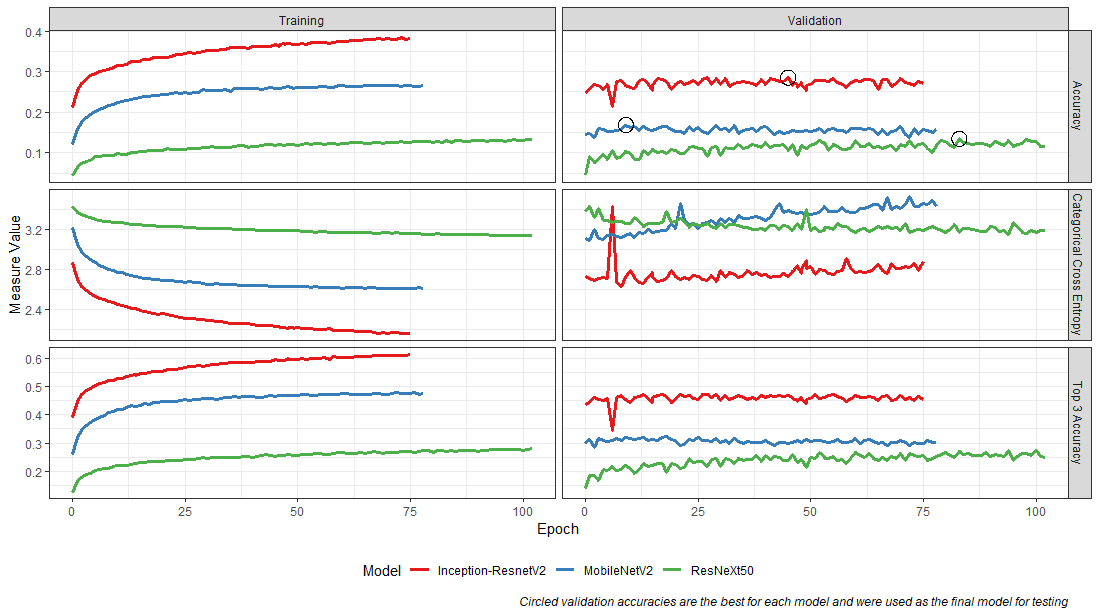
\includegraphics[scale=0.5]{training_results.png}
	\caption{Performance of models on training and validation data throughout training. Note that models that end short stopped training due to early stopping.}
	\label{fig:train_perf}
\end{figure}

Iwana et al. trained their models for 30,000 and 450,000 epochs for LeNet and AlexNet respectively, order of magnitudes more than we trained our models for, so it is likely that the results they achieved are better than they would have been if they had trained for only a few hundred epochs. It is possible, but not certain, that by training our models for a factor of 10 or 100 more epochs, and removing the early stopping criteria, that we could have achieved even better validation performance. 

MobileNetV2 achieved the best validation accuracy early on in its training, where Inception-ResNet-v2 continued to see improvement until just before the 50th epoch, ResNeXt50 sees its best performance coming after the 75th epoch, but as we will see this is not indicative of better performance; the accuracy of ResNeXt50 at any time never improved beyond the lowest accuracy for MobileNetV2 on the training or validation data despite being a more complex model and training for more epochs.
% subsection Training_Performance end 

% section Model_Training end 

\section{Evaluation} 
\label{sec:Evaluation_and_Further_Exploration} 
\subsection{Results} 
\label{sub:Results} 
Full results for all 3 models evaluated on the test set are available in \cref{tab:results_acc}, along with those reported by Iwana for ease of comparison. A visual representation of this for our models only is shown in \cref{fig:test_perf}. As a reminder, the dataset used for our models was slightly altered from the original set, and due to the use of a validation dataset was not trained on the full set of records; but for a comparison it is suitable. Inception-ResNet-v2 is comparable to the results of AlexNet but is slightly more accurate when Top-3 predictions are taken into account. MobileNetV2 is close to LeNet in performance, with just slightly improvements in many genres. ResNeXt50 shows very odd behaviour, with many classes showing near 0\% accuracy even at Top-3, whilst some classes have a very high accuracy such as Biographies and Memoirs. This is likely an artefact of it overlapping specific classes which along with is discussed further in \cref{sub:Further_Analysis}.

At a per-genre level Inception-ResNet-v2 shows the best results on 16 out of the 30 genres for top-1 predictions, followed by 10 for AlexNet. If we further explore the seemingly best performing classes in ResNeXt50 we can see by looking at the precision as presented in \cref{tab:test_prec} that in the genres where this model seems to perform well the precision is low (when compared to for example Inception-ResNet-v2) which provides further evidence that for some classes it combines multiple genres and just predicts one of them i.e. whilst the model is able to correctly predict these \emph{chosen}	classes when it sees them, it is highly likely to predict other genres as one of these as well.

Overall the results from Inception-ResNet-v2 are promising given the low training time and adjusted dataset; the potential improvements are discussed further in \cref{sub:Discussion}.

\begin{table}[]
	\centering
	\resizebox{\textwidth}{!}{%
	\begin{tabular}{lrrrrrrrrrrrrrr}
								   & \multicolumn{2}{c}{\textbf{LeNet*}}                                     & \multicolumn{1}{c}{\textbf{}} & \multicolumn{2}{c}{\textbf{AlexNet*}}                                   & \multicolumn{1}{c}{\textbf{}} & \multicolumn{2}{c}{\textbf{MobileNetV2}}                                & \multicolumn{1}{c}{\textbf{}} & \multicolumn{2}{c}{\textbf{Inception-ResNet-v2}}                         & \multicolumn{1}{c}{\textbf{}} & \multicolumn{2}{c}{\textbf{ResNeXt50}}                                  \\
	\textbf{Genre}                 & \multicolumn{1}{c}{\textbf{Top 1}} & \multicolumn{1}{c}{\textbf{Top 3}} & \multicolumn{1}{c}{\textbf{}} & \multicolumn{1}{c}{\textbf{Top 1}} & \multicolumn{1}{c}{\textbf{Top 3}} & \multicolumn{1}{c}{\textbf{}} & \multicolumn{1}{c}{\textbf{Top 1}} & \multicolumn{1}{c}{\textbf{Top 3}} & \multicolumn{1}{c}{\textbf{}} & \multicolumn{1}{c}{\textbf{Top 1}} & \multicolumn{1}{c}{\textbf{Top 3}} & \multicolumn{1}{c}{\textbf{}} & \multicolumn{1}{c}{\textbf{Top 1}} & \multicolumn{1}{c}{\textbf{Top 3}} \\ \hline
	Arts \& Photography            & 5.8                                & 11.6                               &                               & 12.1                               & 31.1                               &                               & 11.1                               & 27.9                               &                               & \textit{13.2}                      & \textit{33.7}                      &                               & 3.7                                & 11.1                               \\
	Biographies \& Memoirs         & 5.3                                & 18.4                               &                               & 13.2                               & 29.5                               &                               & 10.0                               & 30.5                               &                               & \textit{23.2}                      & 46.3                               &                               & 20.0                               & \textit{60.0}                      \\
	Business \& Money              & 10.0                               & 25.3                               &                               & 12.6                               & 25.8                               &                               & 4.7                                & 18.4                               &                               & \textit{13.2}                      & \textit{33.7}                      &                               & 1.1                                & 3.2                                \\
	Calendars                      & 18.9                               & 37.9                               &                               & \textit{47.9}                      & \textit{65.3}                      &                               & 13.7                               & 25.8                               &                               & 25.8                               & 37.4                               &                               & 18.9                               & 24.7                               \\
	Children’s                     & 24.7                               & 42.1                               &                               & \textit{42.1}                      & \textit{61.6}                      &                               & 30.0                               & 52.1                               &                               & 18.9                               & 43.2                               &                               & 11.6                               & 34.7                               \\
	Comics \& Graphic Novels       & 15.8                               & 33.7                               &                               & 47.4                               & 67.9                               &                               & 40.5                               & 56.8                               &                               & \textit{56.3}                      & \textit{72.6}                      &                               & 47.9                               & 60.5                               \\
	Computers \& Technology        & 29.5                               & 42.8                               &                               & \textit{44.7}                      & \textit{59.5}                      &                               & 28.4                               & 43.7                               &                               & 41.1                               & 57.4                               &                               & 17.9                               & 26.8                               \\
	Cookbooks, Food \& Wine        & 14.2                               & 32.6                               &                               & \textit{43.7}                      & \textit{57.4}                      &                               & 23.7                               & 42.1                               &                               & 40.0                               & 55.8                               &                               & 7.9                                & 23.2                               \\
	Crafts, Hobbies \& Home        & 7.4                                & 22.1                               &                               & 17.4                               & 36.8                               &                               & 13.7                               & 30.5                               &                               & \textit{31.6}                      & \textit{60.0}                      &                               & 2.6                                & 15.3                               \\
	Christian Books \& Bibles      & \textit{8.4}                       & 23.7                               &                               & 7.4                                & \textit{26.3}                      &                               & 2.6                                & 12.1                               &                               & 4.2                                & 20.5                               &                               & 0.0                                & 0.5                                \\
	Engineering \& Transportation  & 10.0                               & 21.1                               &                               & 20.0                               & 34.7                               &                               & 15.3                               & 32.1                               &                               & \textit{20.0}                      & \textit{35.3}                      &                               & 6.8                                & 24.7                               \\
	Health, Fitness \& Dieting     & 4.2                                & 15.8                               &                               & 12.6                               & 29.5                               &                               & 4.2                                & 17.9                               &                               & \textit{12.6}                      & \textit{37.4}                      &                               & 3.7                                & 25.8                               \\
	History                        & 6.3                                & 16.8                               &                               & 12.6                               & 27.9                               &                               & 6.8                                & 21.6                               &                               & \textit{15.8}                      & \textit{38.4}                      &                               & 1.1                                & 2.1                                \\
	Humor \& Entertainment         & 5.3                                & 16.3                               &                               & 10.5                               & 22.6                               &                               & 0.0                                & 7.4                                &                               & \textit{16.3}                      & \textit{43.7}                      &                               & 0.0                                & 2.6                                \\
	Law                            & 14.7                               & 25.8                               &                               & 25.3                               & 38.4                               &                               & 16.3                               & 27.4                               &                               & 17.9                               & 37.9                               &                               & \textit{26.8}                      & \textit{45.3}                      \\
	Literature \& Fiction          & 3.2                                & 12.1                               &                               & \textit{11.1}                      & 22.6                               &                               & 6.3                                & 24.7                               &                               & 10.5                               & \textit{38.9}                      &                               & 0.5                                & 2.6                                \\
	Medical Books                  & 12.6                               & 30.0                               &                               & 19.5                               & 36.8                               &                               & 11.1                               & 27.4                               &                               & \textit{20.0}                      & \textit{45.8}                      &                               & 13.7                               & 38.9                               \\
	Mystery, Thriller \& Suspense  & 23.7                               & 40.0                               &                               & 34.2                               & 48.9                               &                               & 12.1                               & 28.9                               &                               & \textit{34.7}                      & \textit{59.5}                      &                               & 19.5                               & 28.9                               \\
	Parenting \& Relationships     & 14.7                               & 35.3                               &                               & \textit{24.2}                      & 39.5                               &                               & 24.2                               & \textit{43.7}                      &                               & 22.6                               & 42.1                               &                               & 4.7                                & 22.6                               \\
	Politics \& Social Sciences    & 3.7                                & 18.4                               &                               & 6.8                                & 21.6                               &                               & \textit{26.3}                      & \textit{55.8}                      &                               & 2.6                                & 13.2                               &                               & 0.5                                & 12.6                               \\
	Reference                      & 13.2                               & 26.8                               &                               & \textit{20.0}                      & \textit{34.2}                      &                               & 11.1                               & 21.6                               &                               & 8.9                                & 27.9                               &                               & 2.6                                & 18.4                               \\
	Religion \& Spirituality       & 8.4                                & 27.9                               &                               & 16.3                               & 31.6                               &                               & 7.9                                & 26.3                               &                               & \textit{36.3}                      & \textit{55.8}                      &                               & 0.0                                & 0.5                                \\
	Romance                        & 27.4                               & 43.2                               &                               & \textit{45.3}                      & \textit{60.5}                      &                               & 38.4                               & 52.1                               &                               & 40.5                               & 59.5                               &                               & 25.8                               & 52.1                               \\
	Science \& Math                & 8.4                                & 26.3                               &                               & 14.2                               & 29.5                               &                               & 3.7                                & 16.3                               &                               & \textit{26.3}                      & \textit{56.3}                      &                               & 0.0                                & 0.5                                \\
	Science Fiction \& Fantasy     & 14.7                               & 33.2                               &                               & \textit{35.8}                      & 52.6                               &                               & 21.6                               & 42.1                               &                               & 33.7                               & \textit{55.8}                      &                               & 18.9                               & 39.5                               \\
	Self-Help                      & 13.7                               & 31.6                               &                               & 14.2                               & 33.2                               &                               & 3.7                                & 17.9                               &                               & 11.6                               & 28.4                               &                               & \textit{18.9}                      & \textit{46.8}                      \\
	Sports \& Outdoors             & 5.3                                & 16.8                               &                               & 14.7                               & 28.4                               &                               & 1.1                                & 4.7                                &                               & \textit{27.4}                      & \textit{53.2}                      &                               & 0.0                                & 2.1                                \\
	Teen \& Young Adult            & 7.9                                & 17.4                               &                               & 12.1                               & 28.4                               &                               & 7.4                                & 28.9                               &                               & \textit{13.2}                      & \textit{35.3}                      &                               & 0.0                                & 0.5                                \\
	Test Preparation               & 47.9                               & 56.8                               &                               & \textit{68.9}                      & \textit{78.4}                      &                               & 34.2                               & 47.9                               &                               & 56.8                               & 74.2                               &                               & 50.5                               & 66.8                               \\
	Travel                         & 19.5                               & 33.7                               &                               & 33.2                               & 48.4                               &                               & 7.4                                & 14.2                               &                               & \textit{44.7}                      & \textit{64.2}                      &                               & 24.2                               & 41.1                               \\ \hline
	\textbf{Total Accuracy}         & \textbf{13.5}                      & \textbf{27.8}                      & \textbf{}                     & \textbf{24.7}                      & \textbf{40.3}                      & \textbf{}                     & \textbf{14.6}                      & \textbf{30.0}                      &                               & \textit{\textbf{24.7}}             & \textit{\textbf{45.4}}             &                               & \textbf{11.7}                      & \textbf{24.5}                      \\ \hline
	\textit{Number of best genres} & \textit{1}                         & \textit{0}                         & \textit{}                     & \textit{10}                        & \textit{8}                         & \textit{}                     & \textit{1}                         & \textit{2}                         & \textit{}                     & \textit{16}                        & \textit{17}                        & \textit{}                     & \textit{2}                         & \textit{3}                        
	\end{tabular}%
	}
	\caption{Top-1 and -3 Per-class recall (and overall accuracy) for the 3 trained models and the results presented by Iwana for comparison. Italics represent the best result for that genre in Top-1/3 recall/accuracy. \\
	\tiny{*Iwana results are based on a slightly different training and test set}
	}
	\label{tab:results_acc}
	\end{table}


\begin{figure}
	\centering
	\captionsetup{justification=centering}
	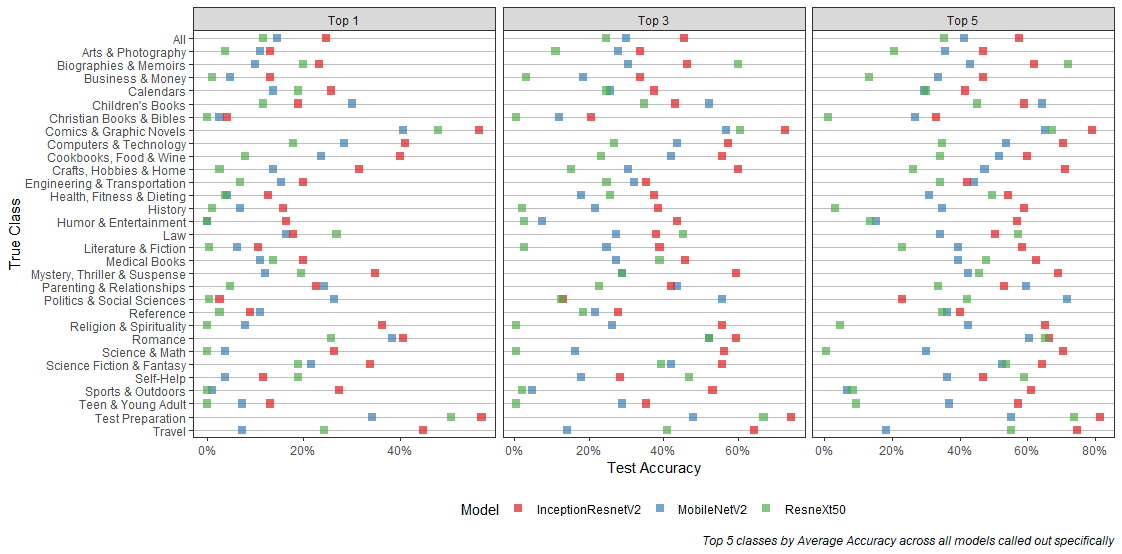
\includegraphics[scale=0.5]{accuracy_by_model.png}
	\caption{Top-1/3/5 recall (accuracy for all) of each model by genre}
	\label{fig:test_perf}
\end{figure}

\begin{table}[]
	\centering
	%\resizebox{\textwidth}{!}{%
	\begin{tabular}{lrrr}
	\textbf{Predicted Genre}      & \multicolumn{1}{c}{\textbf{MobileNetV2}} & \multicolumn{1}{c}{\textbf{Inception-ResNet-v2}} & \multicolumn{1}{c}{\textbf{ResNeXt50}} \\ \hline
	Arts \& Photography           & 17.8                                     & 20.8                                            & 25.9                                   \\
	Biographies \& Memoirs        & 11.5                                     & 19.3                                            & 5.5                                    \\
	Business \& Money             & 11.0                                     & 13.4                                            & 20.0                                   \\
	Calendars                     & 32.5                                     & 31.2                                            & 16.8                                   \\
	Children's Books              & 24.2                                     & 36.7                                            & 13.2                                   \\
	Christian Books \& Bibles     & 5.6                                      & 17.4                                            &                                        \\
	Comics \& Graphic Novels      & 19.7                                     & 46.5                                            & 17.1                                   \\
	Computers \& Technology       & 26.3                                     & 31.1                                            & 19.3                                   \\
	Cookbooks, Food \& Wine       & 19.1                                     & 65.0                                            & 16.3                                   \\
	Crafts, Hobbies \& Home       & 14.2                                     & 27.5                                            & 31.3                                   \\
	Engineering \& Transportation & 10.2                                     & 54.3                                            & 12.3                                   \\
	Health, Fitness \& Dieting    & 5.9                                      & 15.2                                            & 5.9                                    \\
	History                       & 13.5                                     & 20.3                                            & 66.7                                   \\
	Humor \& Entertainment        & 0.0                                      & 13.4                                            & 0.0                                    \\
	Law                           & 16.1                                     & 24.1                                            & 9.4                                    \\
	Literature \& Fiction         & 8.7                                      & 11.6                                            & 50.0                                   \\
	Medical Books                 & 12.4                                     & 16.5                                            & 12.5                                   \\
	Mystery, Thriller \& Suspense & 25.8                                     & 23.8                                            & 19.5                                   \\
	Parenting \& Relationships    & 9.8                                      & 33.9                                            & 8.2                                    \\
	Politics \& Social Sciences   & 5.5                                      & 11.1                                            & 5.3                                    \\
	Reference                     & 19.4                                     & 26.2                                            & 10.2                                   \\
	Religion \& Spirituality      & 9.6                                      & 16.7                                            &                                        \\
	Romance                       & 14.6                                     & 44.0                                            & 14.0                                   \\
	Science \& Math               & 11.9                                     & 11.8                                            & 0.0                                    \\
	Science Fiction \& Fantasy    & 18.3                                     & 39.5                                            & 13.6                                   \\
	Self Help                     & 12.3                                     & 22.9                                            & 7.2                                    \\
	Sports \& Outdoors            & 22.2                                     & 26.0                                            & 0.0                                    \\
	Teen \& Young Adult           & 9.5                                      & 14.2                                            & 0.0                                    \\
	Test Preparation              & 50.4                                     & 43.7                                            & 13.0                                   \\
	Travel                        & 50.0                                     & 17.3                                            & 8.3                                    \\ \hline
	\textbf{Total Precision}      & \textbf{14.6}                            & \textbf{24.7}                                   & \textbf{11.7}                          \\ \hline
	\end{tabular}%
	%}
	\caption{Top-1 Per class, and total, precision for each model \\ \tiny{Missing values represent no predictions made in that class over the test set}}
	\label{tab:test_prec}
	\end{table}

% section Results end 
\subsection{Further Analysis} 
\label{sub:Further_Analysis} 
In the paper by Iwana they discuss the potential reasons for the disparity between the recall by genre and investigate some examples. They call out consistency of colour, objects, and text styles are key elements that impact the ability for a genre to be able to be predicted well by their models. Here we focus on the colour component as the strongest driver for predictability and investigate the ways in which the models may be driven by colour of the cover images.

First, as displayed in \cref{fig:col_distributions}, we can see that whilst there is a wide range of average RGB values and width/aspect ratio (height is almost entirely consistent across genres), there are no standout values in colour alone that allow for easy genre classification. Width/aspect ratio, something that wasn't directly included in the model (but was indirectly by the use of the padding applied during the pre-processing), contains some clearer distinctions; in particular Calendars have a very different distribution of aspect ratios compared to other genres, and children books contains some wider books when compared to other categories. Whilst none of this alone would be enough to provide good classification, it does suggest that explicit inclusion of dimensional information in a model could improve the performance when combined with the existing output. 

\begin{figure}
	\centering
	\captionsetup{justification=centering}
	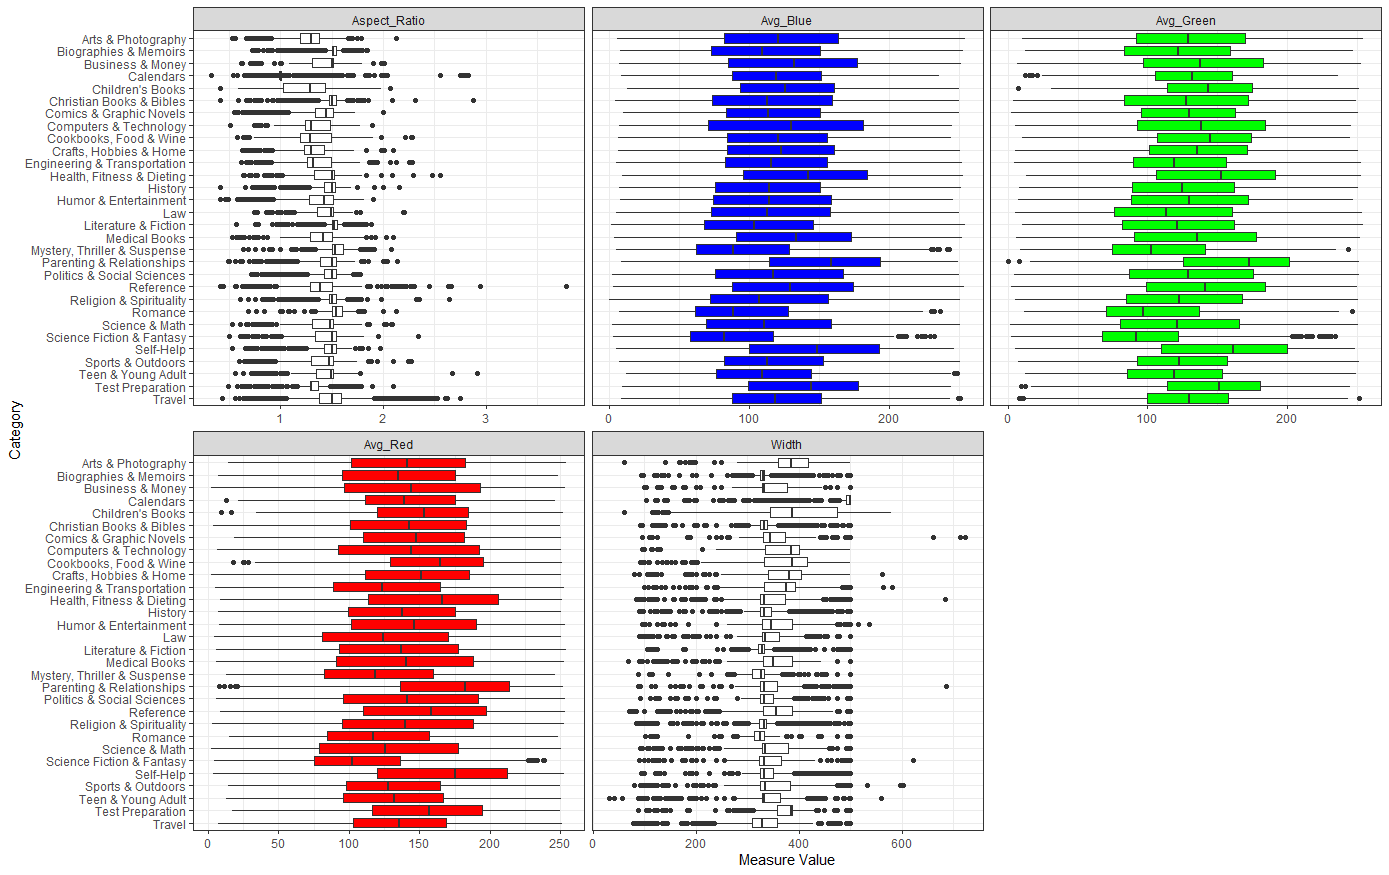
\includegraphics[scale=0.45]{distributions_col_ratio.png}
	\caption{Distributions of various measures by genre}
	\label{fig:col_distributions}
\end{figure}

The average overall colour per genre is presented in \cref{fig:avg_col} which does suggest some slight differences between the genres; similar to the callouts made by Iwana, Sci-Fi and Fantasy seem to be darker when compared to something like Cookbooks, Food and Wine. We can compare the average colour of the true classes against those predicted by each model and visualise how these correlate with the accuracy per class as shown in \cref{fig:col_distance}. Here the colour distance is defined as 

\begin{equation}
	d_{colour} = \sqrt{(R_2 - R_1)^2 + (G_2 - G_1)^2 +(B_2 - B_1)^2 }
\end{equation}
where R/G/B are the average red, green, and blue values for each predicted and true class respectively. We can see a small trends here, particular in MobileNetV2, where the closer the average colour of the true class the better the recall of that class. This is of course a somewhat self-fulfilling prophecy; the more you correctly predict the class the more the dataset will be the true class, however it highlights that even by just guessing based on closeness to average colour you can make some small improvements. This supports the claims made by Iwana in their work. 


\begin{figure}
	\centering
	\captionsetup{justification=centering}
	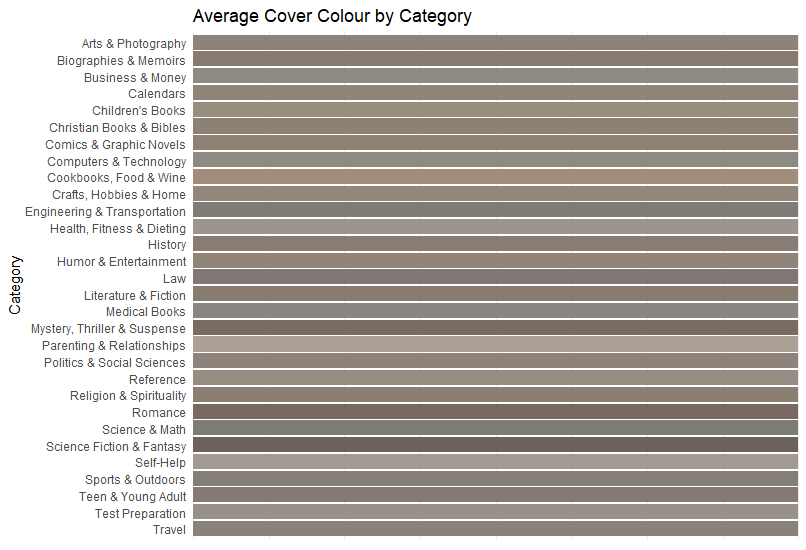
\includegraphics[scale=0.45]{avg_col_plot.png}
	\caption{Average cover colour by genre}
	\label{fig:avg_col}
\end{figure}

\begin{figure}
	\centering
	\captionsetup{justification=centering}
	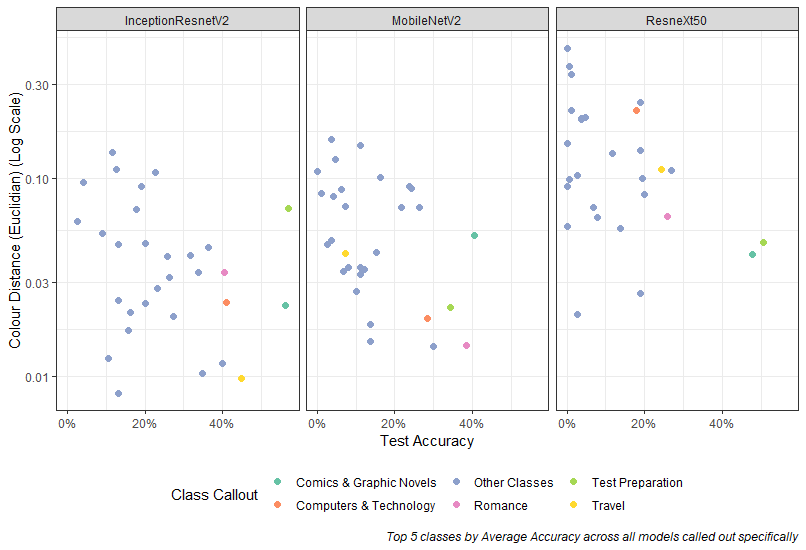
\includegraphics[scale=0.6]{col_dist_plot.png}
	\caption{Colour Distance vs Recall per genre by model}
	\label{fig:col_distance}
\end{figure}

Finally, we can review the \emph{class overlap} for each model. We define class overlap between class A and B for a single prediction as the ratio of the probability of prediction for class A and class B (where B has a higher probability) i.e.
\begin{equation}
	CO(A, B) \stackrel{\mathrm{def}}{=} \min\left\{\frac{P(A)}{P(B)}, \frac{P(B)}{P(A)}\right\}
\end{equation}
The per genre pair class overlap is defined as the average class overlap across all predictions. As we can see in \cref{fig:class_overlap}, where only class overlaps of greater than 0.5 are displayed, the ResNeXt50 model sees large amounts of class overlap between many classes, which agrees with what we saw before that certain classes were being \emph{confused} for each other by the model. Comparatively, MobileNetV2 sees only a few class overlaps greater than 0.5 and Inception-ResNet-v2 sees none. When we examine those with higher overlap in MobileNetV2 we can begin to understand the potential true overlap between classes; \emph{Self-Help} has overlap with \emph{Health, Fitness and Dieting,} \emph{Science and Maths} has overlap with \emph{Medical Books}, and \emph{Religion and Spirituality} has overlap with \emph{Christian Books and Bibles}. All of these are logical overlaps and were a human tasked with classifying books based on their cover into these categories it is highly probable that different people would classify them differently. 

\begin{figure}
	\centering
	\captionsetup{justification=centering}
	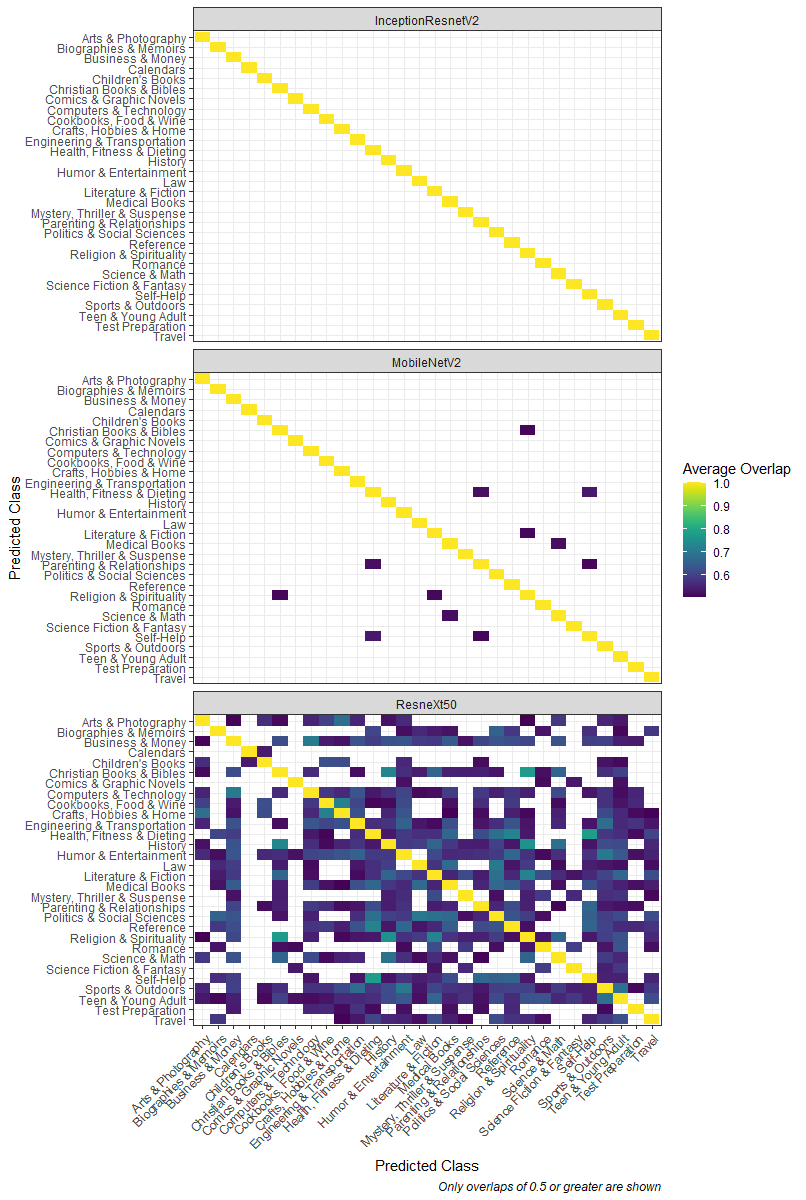
\includegraphics[scale=0.6]{class_pred_overlap.png}
	\caption{Average class overlap by model}
	\label{fig:class_overlap}
\end{figure}
% section Further_Analysis end 
\subsection{Feature Visualisation} 
\label{sub:Feature_Visualisation} 
The goal of using feature visualisation was to attempt to understand what, if any, underlying structure or information the models were using to aid their classification. To do this we use activation maximisation as implemented into the python package \emph{tf-keras-vis}\cite{keras-vis} to do the computational work. To produce the images the final layer activation function was changed from softmax to linear to ensure that target class is being visualised as opposed to just minimising minimising other class activations, and the loss function is simply defined as that linear activation (note here that loss is really a misnomer as we are trying to maximise this value as opposed to minimise it as we traditionally would) as discussed in \cref{sub:Activation_Maximisation}. L2 normalisation was used as the default to attempt to avoid pure static images being produced.

We ran the activation maximisation on the Inception-ResNet-v2 model for the 3 best predicted genres (Test Prep, Comics \& Graphic Novels, and Travel) as we believed these had the best probability of returning useful images. The inputs to the model were then trained for 1000 epochs, at which point issues were encountered with the RAM on the machine. During these steps there was some improvement to the loss function however did not appear to converge. When compared to the progress seen on a pure ImageNet model these saw very little movement and remained negative the entire time (where as the examples provided by the package are always positive after the first few epochs). Even when all regularisation terms were removed, allowing the process to fully maximise the activation without constraints we still did not see an improvement in the loss values.

The results of this attempt can be seen in \cref{fig:act_max_output} and whilst it may be possible to argue that there are some differences between these images that you could prescribe to the common layout of these type of genres covers, it would be difficult to say this with any conviction. Overall the images are generic and provided no additional insight to understand what features the model is identifying to use for the classification.

\begin{figure}
	\centering
	\captionsetup{justification=centering}
	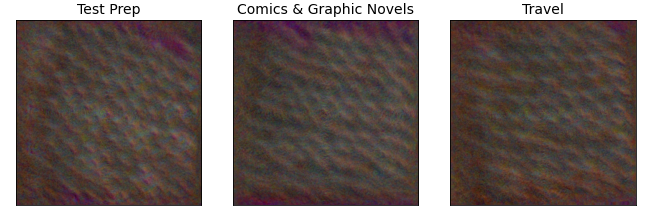
\includegraphics[scale=0.6]{visualize-dense-layer.png}
	\caption{Activation maximisation outputs for the 3 best predicted classes of the Inception-ResNet-v2 model}
	\label{fig:act_max_output}
\end{figure}
% section Feature_Visualisation end  

\subsection{Discussion \& Future Work} 
\label{sub:Discussion} 
Overall the Inception-ResNet-v2 model provided the best results of the 3 models we tried, however it is far more complex than AlexNet but did not provide greatly improved results. The counterpoint to this is that the AlexNet model as trained by Iwana et al. was trained for 450,000 epochs where our model was trained for less than 50 epochs total. We do not know the progress of the training of the model by Iwana but it would be reasonable to suggest that if their model had trained for less epochs, or ours for more, then there would be a greater difference between the results. Despite training on slightly less data (due to the validation set), we can see that more modern and powerful CNNs are able to predict book genres with slightly improved accuracy compared to older methods.

There are lots of directions this work could continue to go in the future; as mentioned before there is still more investigation that can be done surrounding the pre-processing of data, either varying the interpolation methods for downsizing or re-testing the pre-processing methods used specifically on the end model architecture for a longer period of time. Our models could be trained for more epochs with a greater requirement on early stopping to allow for long term improvements to be made that may not be evident over a few hundred epochs. Also, additional information such as the width and height or just aspect ratio could be passed to the model as well in an attempt to improve accuracy this way. The final fully connected part of the network could also be increased in complexity to contain more layers as opposed to just the single layer used in our work.

If resources were no constraint some of the larger improvements to the work would be to tune the hyperparameters of the model, and even train the actual core part of the architecture itself rather than relying entirely on transfer learning and freezing the weights for this component. To do this would require a far greater dataset of images so a generator may have to be used or a larger dataset collected first. Finally, as shown by the results in \cref{tab:results_acc} there is not a single model that performs best across all genres, so an ensemble method may be able to increase the accuracy at the cost of increased complexity. Many of these suggestions are beyond the scope of many citizen data scientists resources and would also lead to a model that may have a prediction time that makes it prohibitive for any real-time use.
% subsection Discussion end 
% section Evaluation_and_Further_Exploration end 

\section{Conclusion} 
\label{sec:Conclusion} 
In this work we have attempted to improve on the work of Iwana et al. and better answer the question can a CNN judge a book by its cover. We reprocessed the dataset initially collected by Iwana and applied multiple pre-processing techniques in an attempt to identify the best method to deal with the impact of different shaped images. We then proceeded to train 3 modern models via transfer learning on a padded version of the dataset and evaluated the results. Finally we attempted to produce ideal class images using activation maximisation for the best model and genres.

We have seen that by using a more modern CNN architecture, namely Inception-ResNet-v2, we are able to improve on the results published by Iwana slightly, whilst training for substantially less epochs. We have also provided some further supporting insight into the components that factor into book cover design i.e. colour, and identified where classifications are failing where this might be due to overlap between classes.

There is still lots to explore in this space as we discussed in \cref{sub:Discussion} and hopefully this work provides a springboard to enable more complex CNNs to be used for genre identification of book covers in the future. The work itself is unlikely to provide any value for real-world use as the accuracy is too low to be of use for either consumers or even cover designers as a form of QA. Genre prediction from cover images remains a complex topic and given the subjectivity of the classifications is unlikely to ever be fully solved, however the work produced here gets a little closer than we were before. So it seems for now that, if you are a CNN, you should follow the old adage and don't judge a book by its cover.
% section Conclusion end 

%\nocite{*}
\bibliographystyle{ieeetran}
\bibliography{BBK_MSc_Project} 

\appendix

\section{CNN Architectures} 
\label{sec:CNN_Architectures} 
Detail the exact configurations of these architectures
\subsection{MobileNetV2} 
\label{sub:MobileNetV2} 
Full technical details of the specification is available in the paper by Sandler at al. \cite{Sandler2018} where the model is first published. The version we use is identical using the Keras implementation with the exception that we do not use a final Conv2D layer but instead use a dense fully connected layer of size 30 to use for our classification. The table and captions explaining the architecture is copied from their paper to here for convenience. The only other difference not detailed in these tables is batch normalisation is applied after each convolution but before the ReLU, and zero padding is applied where a stride of 2 is used. 


\begin{table}[H]
	\centering
	\begin{tabular}{c|c|c}
	\hline
	\textbf{Input}                            & \textbf{Operator}           & \textbf{Output}                            \\ \hline \hline
	$h \times w \times k$                     & 1x1 conv2d, ReLU6           & $h \times w \times tk$                     \\
	$h \times w \times tk$                    & 3x3 dwise stride=$s$, ReLU6 & $\frac{h}{s} \times \frac{w}{s} \times k$  \\
	$\frac{h}{s} \times \frac{w}{s} \times k$ & linear 1x1 covn2d           & $\frac{h}{s} \times \frac{w}{s} \times k'$ \\ \hline
	Iff $s \equiv 1$ \& $k \equiv k'$ then $h \times w \times k$ & add original input           & $h \times w \times k'$ \\ \hline
	\end{tabular}
	\caption{Bottleneck residual block transforming from $k$ to $k'$ channels, with stride $s$, and expansion factor $t$.
	}
	\label{tab:bottleneck}
	\end{table}

\begin{table}[H]
	\centering
	\begin{tabular}{c|c|c|c|c|c}
	\hline
	\textbf{Input}         & \textbf{Operator} & \textbf{t} & \textbf{c} & \textbf{n} & \textbf{s} \\ \hline \hline
	$224^2$ $\times$ 3         & conv2d, ReLU6           & -          & 32         & 1          & 2          \\
	$112^2$ $\times$ 32        & bottleneck        & 1          & 16         & 1          & 1          \\
	$112^2$ $\times$ 16        & bottleneck        & 6          & 24         & 2          & 2          \\
	$56^2$ $\times$ 24         & bottleneck        & 6          & 32         & 3          & 2          \\
	$28^2$ $\times$ 32         & bottleneck        & 6          & 64         & 4          & 2          \\
	$14^2$ $\times$ 64         & bottleneck        & 6          & 96         & 3          & 1          \\
	$14^2$ $\times$ 96         & bottleneck        & 6          & 160        & 3          & 2          \\
	$7^2$ $\times$ 190         & bottleneck        & 6          & 320        & 1          & 1          \\
	$7^2$ $\times$ 320         & conv2d 1x1, ReLU        & -          & 1280       & 1          & 1          \\
	$7^2$ $\times$ 1280        & avgpool 7x7       & -          & -          & 1          & -          \\
	1 $\times$ 1 $\times$ 1280 & dense             & -          & 30         & -          & -          \\ \hline
	\end{tabular}%
	\caption{MobileNetV2 : Each line describes a sequence of 1 or more identical (modulo stride) layers, repeated n times. All layers in the same sequence have the same number c of output channels. The first layer of each sequence has a stride s and all others use stride 1. All
	spatial convolutions use 3 x 3 kernels. The expansion factor t is always applied to the input size as described in \cref{tab:bottleneck}.
	}
	\label{tab:mobilenetv2_arch}
	\end{table}

% subsection MobileNetV2 end  
\subsection{Inception-ResNet-v2} 
\label{sub:Inception-ResnetV2} 
The architecture, with all the relevant filter and stride settings are detailed within the original paper by Szegedy et al. \cite{Szegedy2016} however the Keras implementation seems to differ slightly and the original paper does not provide a full spec in a single place so it is composed here. For simplicity batch normalisation is not explicitly written but is used after every convolution operator and ReLU activation is used throughout. A summarised version is available in \cref{fig:incepresnetv2}\cite{Alemi2016}.


\begin{figure}[H]
	\centering
	\captionsetup{justification=centering}
	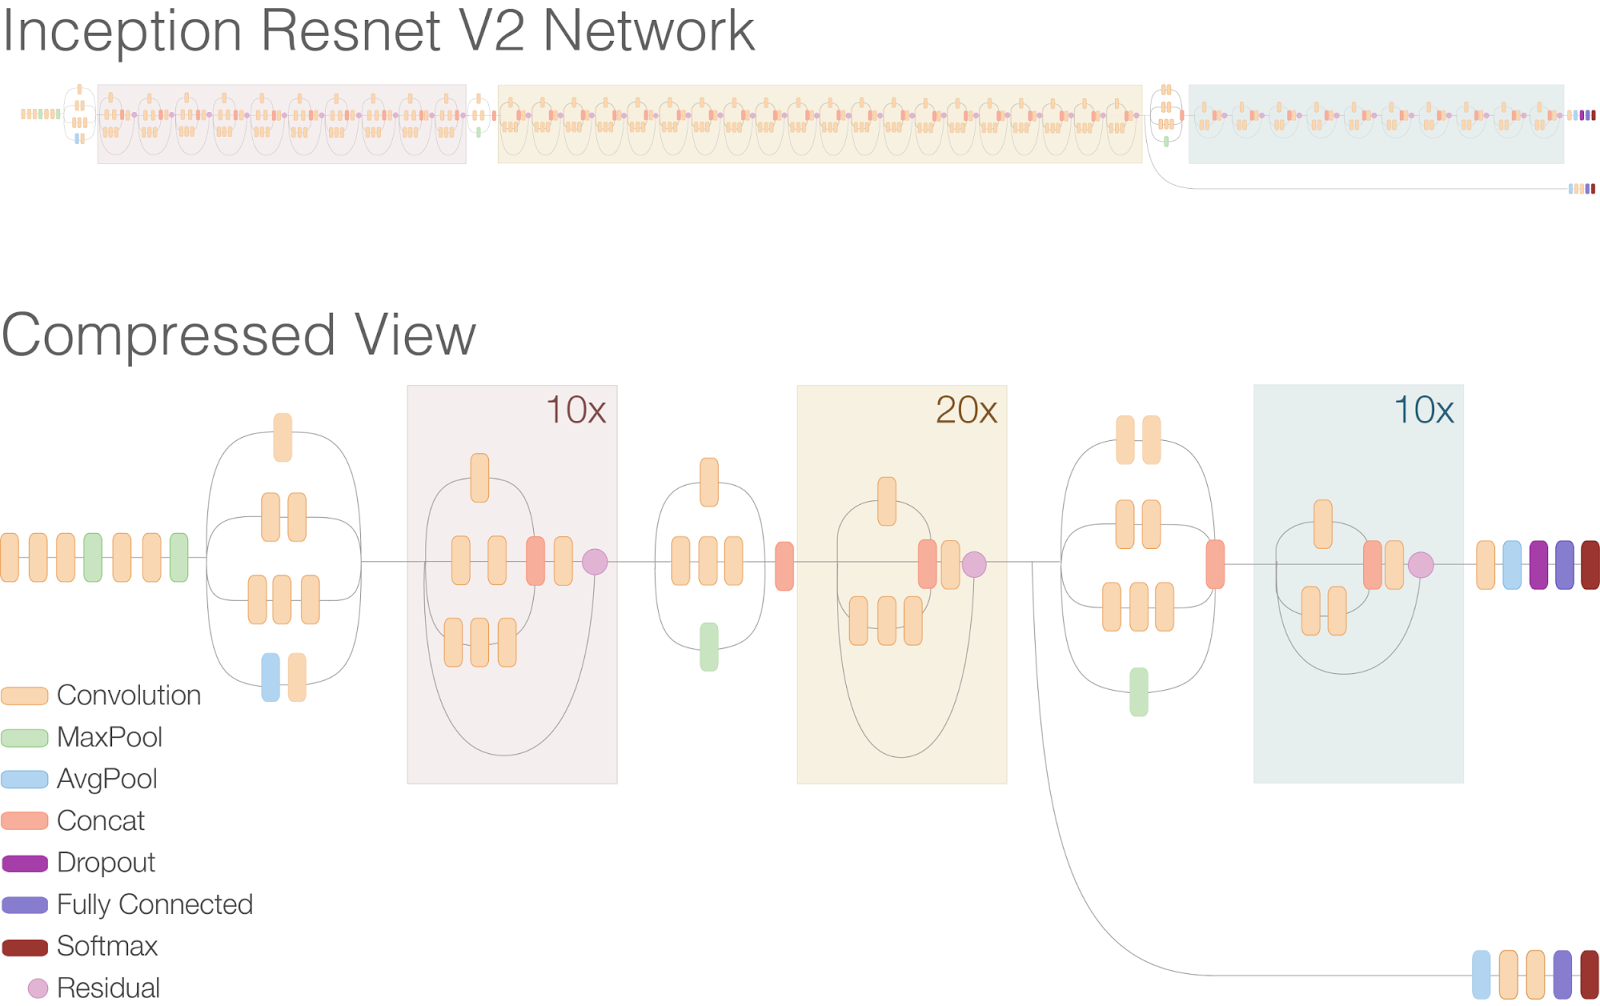
\includegraphics[scale=0.25]{inception_resnetv2.png}
	\caption{High level view of the Inception-ResNet-v2 architecture. The early classifier (bottom of image) is not used in our work.}
	\label{fig:incepresnetv2}
\end{figure}



\begin{table}[H]
	\centering
	\resizebox{\textwidth}{!}{%
	\begin{tabular}{c|c|c|c|c|c|c}
	\textbf{Block Name}      & \textbf{LayerID} & \textbf{Input} & \textbf{Operator} & \textbf{Filters} & \textbf{Shape} & \textbf{Scale} \\ \hline \hline
	Inception-ResNet-A block & 0                & -              & conv2d            & 32               & 1              & -              \\
	Inception-ResNet-A block & 1                & -              & conv2d            & 32               & 1              & -              \\
	Inception-ResNet-A block & 2                & 1              & conv2d            & 32               & 3              & -              \\
	Inception-ResNet-A block & 3                & -              & conv2d            & 32               & 1              & -              \\
	Inception-ResNet-A block & 4                & 3              & conv2d            & 48               & 3              & -              \\
	Inception-ResNet-A block & 5                & 4              & conv2d            & 64               & 3              & -              \\
	Inception-ResNet-A block & 6                & 0, 2, 5        & concat            & -                & -              & -              \\
	Inception-ResNet-A block & 7                & -, 6           & add w/ scale      & -                & -              & (1, 0.17) \\ \hline  
	\end{tabular}
	}
	\caption{Structure of the Inception-ResNet-A block. Shape unless otherwise specified is square, and scale is the multiplier of the inputs of the addition. - in input represents the input to the block.}
	\label{tab:incepresa}
	\end{table}

\begin{table}[H]
	\centering
	\resizebox{\textwidth}{!}{%
	\begin{tabular}{c|c|c|c|c|c|c}
	\textbf{Block Name}        & \textbf{LayerID} & \textbf{Input} & \textbf{Operator} & \textbf{Filters} & \textbf{Shape} & \textbf{Scale} \\ \hline \hline
	Inception-ResNet-B block & 0                & -              & conv2d            & 192              & 1              & -              \\
	Inception-ResNet-B block   & 1                & -              & conv2d            & 128              & 1              & -              \\
	Inception-ResNet-B block   & 2                & 1              & conv2d            & 160              & (1, 7)         & -              \\
	Inception-ResNet-B block   & 3                & 2              & conv2d            & 192              & (7, 1)         & -              \\
	Inception-ResNet-B block   & 4                & 0, 3           & concat            & -                & -              & -              \\
	Inception-ResNet-B block   & 5                & `-, 4          & add w/ scale      & -                & -              & (1, 0.1)     \\ \hline  
	\end{tabular}%
	}
	\caption{Structure of the Inception-ResNet-B block. Shape unless otherwise specified is square, and scale is the multiplier of the inputs of the addition. - in input represents the input to the block.}
	\label{tab:incepresb}
	\end{table}

\begin{table}[H]
	\centering
	\resizebox{\textwidth}{!}{%
	\begin{tabular}{c|c|c|c|c|c|c}
	\textbf{Block Name}      & \textbf{LayerID} & \textbf{Input} & \textbf{Operator} & \textbf{Filters} & \textbf{Shape} & \textbf{Scale} \\ \hline \hline
	Inception-ResNet-C block & 0                & -              & conv2d            & 192              & 1              & -              \\
	Inception-ResNet-C block & 1                & -              & conv2d            & 192              & 1              & -              \\
	Inception-ResNet-C block & 2                & 1              & conv2d            & 224              & (1, 3)         & -              \\
	Inception-ResNet-C block & 3                & 2              & conv2d            & 256              & (3, 1)         & -              \\
	Inception-ResNet-C block & 4                & 0, 3           & concat            & -                & -              & -              \\
	Inception-ResNet-C block & 5                & `-, 4          & add w/ scale      & -                & -              & (1, 1) \\ \hline  
	\end{tabular}%
	}
	\caption{Structure of the Inception-ResNet-C block. Shape unless otherwise specified is square, and scale is the multiplier of the inputs of the addition. - in input represents the input to the block.}
	\label{tab:incepresc}
	\end{table}
	
\begin{table}[H]
	\centering
	\resizebox{\textwidth}{!}{%
	\begin{tabular}{c|c|c|c|c|c|c|c}
	\textbf{Block Name}               & \textbf{LayerID} & \textbf{Input} & \textbf{Operator} & \textbf{Filters} & \textbf{Shape} & \textbf{Strides}       & \textbf{N} \\ \hline\hline
	Stem                              & 0                & -              & conv2d            & 32               & 3              & 2                      & 1          \\
	Stem                              & 1                & 0              & conv2d            & 32               & 3              & 1                      & 1          \\
	Stem                              & 2                & 1              & conv2d            & 64               & 3              & 1                      & 1          \\
	Stem                              & 3                & 2              & maxpooling        & -                & 3              & 2                      & 1          \\
	Stem                              & 4                & 3              & conv2d            & 80               & 1              & 1                      & 1          \\
	Stem                              & 5                & 4              & conv2d            & 192              & 3              & 1                      & 1          \\
	Stem                              & 6                & 5              & maxpooling        & -                & 3              & 2                      & 1          \\\hdashline
	Inception-A block                 & 7                & 6              & conv2d            & 96               & 1              & 1                      & 1          \\
	Inception-A block                 & 8                & 6              & conv2d            & 48               & 1              & 1                      & 1          \\
	Inception-A block                 & 9                & 8              & conv2d            & 64               & 5              & 1                      & 1          \\
	Inception-A block                 & 10               & 6              & conv2d            & 64               & 1              & 1                      & 1          \\
	Inception-A block                 & 11               & 10             & conv2d            & 96               & 3              & 1                      & 1          \\
	Inception-A block                 & 12               & 11             & conv2d            & 96               & 3              & 1                      & 1          \\
	Inception-A block                 & 13               & 6              & avgpooling        & -                & 3              & 1                      & 1          \\
	Inception-A block                 & 14               & 13             & conv2d            & 64               & 1              & 1                      & 1          \\
	Inception-A block                 & 15               & 7, 9, 12, 14   & concat            & -                & -              & -                      & -          \\\hdashline
	\textit{Inception-ResNet-A block} & 16               & 15             & -                 & -                & -              & -                      & 10         \\\hdashline
	Reduction-A block                 & 17               & 16             & conv2d            & 384              & 3              & 2                      & 1          \\
	Reduction-A block                 & 18               & 16             & conv2d            & 256              & 1              & 1                      & 1          \\
	Reduction-A block                 & 19               & 18             & conv2d            & 256              & 3              & 1                      & 1          \\
	Reduction-A block                 & 20               & 19             & conv2d            & 284              & 3              & 2                      & 1          \\
	Reduction-A block                 & 21               & 16             & maxpooling        & -                & 3              & 2                      & 1          \\
	Reduction-A block                 & 23               & 17, 20, 21     & concat            & -                & -              & -                      & -          \\\hdashline
	\textit{Inception-ResNet-B block} & 24               & 23             & -                 & -                & -              & -                      & 20         \\
	Reduction-B block                 & 25               & 24             & conv2d            & 256              & 1              & 1                      & 1          \\
	Reduction-B block                 & 26               & 25             & conv2d            & 384              & 3              & 2                      & 1          \\
	Reduction-B block                 & 27               & 24             & conv2d            & 256              & 1              & 1                      & 1          \\
	Reduction-B block                 & 28               & 27             & conv2d            & 288              & 3              & 2                      & 1          \\
	Reduction-B block                 & 29               & 24             & conv2d            & 256              & 1              & 1                      & 1          \\
	Reduction-B block                 & 30               & 29             & conv2d            & 288              & 3              & 1                      & 1          \\
	Reduction-B block                 & 31               & 30             & conv2d            & 230              & 3              & 2                      & 1          \\
	Reduction-B block                 & 32               & 29             & maxpooling        & -                & 3              & 2                      & 1          \\
	Reduction-B block                 & 33               & 26, 28, 31, 32 & concat            & -                & -              & -                      & -          \\\hdashline
	\textit{Inception-ResNet-C block} & 34               & 33             & -                 & -                & -              & -                      & 10         \\\hdashline
	Final convolution block           & 35               & 34             & conv2d            & 1536             & 1              & 1                      & 1          \\
	Global Pooling                    & 36               & 35             & avgpooling        & -                & -              & -                      & -          \\
	Dense                             & 37               & 36             & dense (30)        & -                & -              & - 				& -          \\ \hline
	\end{tabular}%
	}
	\caption{Structure of the Inception-ResNet-v2 model. Shape unless otherwise specified is square, and N is the number of times that layer or block is repeated. For information on the Inception-ResNet blocks see \cref{tab:incepresa,tab:incepresb,tab:incepresc}.  - represents a non-relevant argument or in the case of input, the input to the model.}
	\label{tab:incepresfull}
	\end{table}

% subsection Inception-ResNet-v2 end 
\subsection{ResNeXt50} 
\label{sub:ResNeXt50} 
The full details of the ResNeXt50 architecture and in what way it differs from and improves upon regular ResNets is available in the paper by Xie et al.\cite{Xie2016}. We reproduce here the table (\cref{tab:resnextarc})explaining the architecture and an image (\cref{fig:resnextblocks}) explaining the blocks from their paper for convenience. These models differ in their use of a \emph{cardinality} term, C. This is defined as the number of times a repeated series of convolutional filters in parallel with the exact same parameters are used within a block. All layers are followed by batch normalisation and ReLU activation.


\begin{table}[H]
	\centering
	\resizebox{\textwidth}{!}{%
	\begin{tabular}{c|c|c|c|c|c|c|c}
	\textbf{Stage}         & \textbf{Output}                 & \textbf{Operation}                                                                   & \textbf{Filters} & \textbf{Shape} & \textbf{Stride} & \textbf{Cardinality (C)} & \textbf{N}         \\ \hline \hline
	conv1                  & $112 \times 112$                & conv2d                                                                               & 64               & 7              & 2               & 1                        & 1                  \\ \hline
	\multirow{4}{*}{conv2} & \multirow{4}{*}{$56 \times 56$} & max pooling                                                                          & -                & 3              & 2               & 1                        & 1                  \\ \cline{3-8} 
						   &                                 & \multirow{3}{*}{ResNext Block}                                                       & 128              & 1              & 1               & 1                        & \multirow{3}{*}{3} \\ \cline{4-7}
						   &                                 &                                                                                      & 128              & 3              & 1               & 32                       &                    \\ \cline{4-7}
						   &                                 &                                                                                      & 256              & 1              & 1               & 1                        &                    \\ \hline
	\multirow{3}{*}{conv3} & \multirow{3}{*}{$28 \times 28$} & \multirow{3}{*}{ResNext Block}                                                       & 256              & 1              & 1               & 1                        & \multirow{3}{*}{4} \\ \cline{4-7}
						   &                                 &                                                                                      & 256              & 3              & 1               & 32                       &                    \\ \cline{4-7}
						   &                                 &                                                                                      & 512              & 1              & 1               & 1                        &                    \\ \hline
	\multirow{3}{*}{conv4} & \multirow{3}{*}{$14 \times 14$} & \multirow{3}{*}{ResNext Block}                                                       & 512              & 1              & 1               & 1                        & \multirow{3}{*}{6} \\ \cline{4-7}
						   &                                 &                                                                                      & 512              & 3              & 1               & 32                       &                    \\ \cline{4-7}
						   &                                 &                                                                                      & 1024             & 1              & 1               & 1                        &                    \\ \hline
	\multirow{3}{*}{conv5} & \multirow{3}{*}{$7 \times 7$}   & \multirow{3}{*}{ResNext Block}                                                       & 1024             & 1              & 1               & 1                        & \multirow{3}{*}{3} \\ \cline{4-7}
						   &                                 &                                                                                      & 1024             & 3              & 1               & 32                       &                    \\ \cline{4-7}
						   &                                 &                                                                                      & 2048             & 1              & 1               & 1                        &                    \\ \hline
						   & $1 \times 1$                    & \begin{tabular}[c]{@{}c@{}}global average pooling\\ dense (30), softmax\end{tabular} & -                & -              & -               & 1                        & 1                  \\ \hline
	\end{tabular}%
	}
	\caption{Structure of the ResNeXt50 model. At the end of each block the input is added in (as with the original resnet models) - see example methods in \cref{fig:resnextblocks}.}
	\label{tab:resnextarc}
	\end{table}

	\begin{figure}[H]
		\centering
		\captionsetup{justification=centering}
		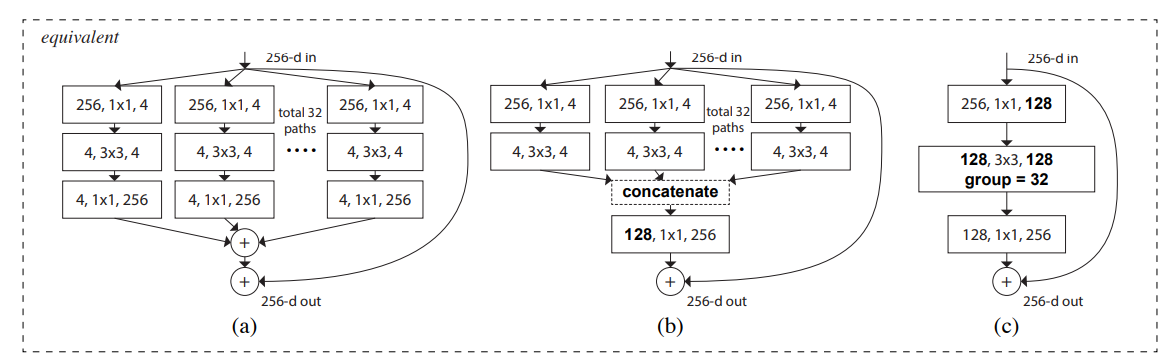
\includegraphics[scale=0.5]{resnextblocks.PNG}
		\caption{\cite{Xie2016} Equivalent methods for each ResNeXt block highlighting the inclusion of the input \emph{shortcut} path as part of the output. In our work the rightmost option was used.}
		\label{fig:resnextblocks}
	\end{figure}
% subsection ResNeXt50 end 
% section CNN_Architectures end 

\section{Technology} 
\label{sec:Technology}
Due to the use of Google Colab for the vast majority of the work is it not possible to confirm which hardware was used over the course of the work, or even that the same was used over multiple sessions.
Software and library versions:
\begin{itemize}
	\item Python: 3.6.9 (linux environment on Google Colab)
	\begin{itemize}
		\item argparse: 1.1 
		\item classification\_model: 0.2.2 
		\item IPython: 5.5.0 
		\item joblib: 0.16.0 
		\item matplotlib: 3.2.2 
		\item skimage: 0.16.2 
		\item sklearn: 0.22.2.post1 
		\item tf\_keras\_vis: 0.5.2 
		\item tqdm: 4.41.1 
		\item cv2: 4.1.2 
		\item numpy: 1.18.5 
		\item pandas: 1.0.5 
		\item re: 2.2.1 
		\item tensorflow: 2.3.0
	\end{itemize}
	\item R: 4.0.0 (64-bit windows)
	\begin{itemize}
		\item ggforce: 0.3.2
		\item tidyr: 1.1.0
		\item ggplot2: 3.3.0
		\item dplyr: 0.8.5
		\item Rcpp: 1.0.4.6
		\item rstudioapi: 0.11
		\item magrittr: 1.5
		\item MASS: 7.3-51.5
		\item tidyselect: 1.1.0
		\item munsell: 0.5.0
		\item viridisLite: 0.3.0
		\item colorspace: 1.4-1
		\item R6: 2.4.1
		\item rlang: 0.4.6
		\item fansi: 0.4.1
		\item tools: 4.0.0
		\item grid: 4.0.0
		\item gtable: 0.3.0
		\item cli: 2.0.2
		\item clipr: 0.7.0
		\item withr: 2.2.0
		\item ellipsis: 0.3.0
		\item assertthat: 0.2.1
		\item tibble: 3.0.1
		\item lifecycle: 0.2.0
		\item crayon: 1.3.4
		\item gridExtra: 2.3
		\item farver: 2.0.3
		\item tweenr: 1.0.1
		\item purrr: 0.3.4
		\item viridis: 0.5.1
		\item vctrs: 0.3.0
		\item glue: 1.4.0
		\item polyclip: 1.10-0
		\item stringi: 1.4.6
		\item compiler: 4.0.0
		\item pillar: 1.4.4
		\item scales: 1.1.1
		\item pkgconfig: 2.0.3
	\end{itemize}
\end{itemize}
% section Technology end 
\end{document}